\documentclass{standalone}
\usepackage{mathpazo}
\usepackage[american]{circuitikz}

\begin{document}
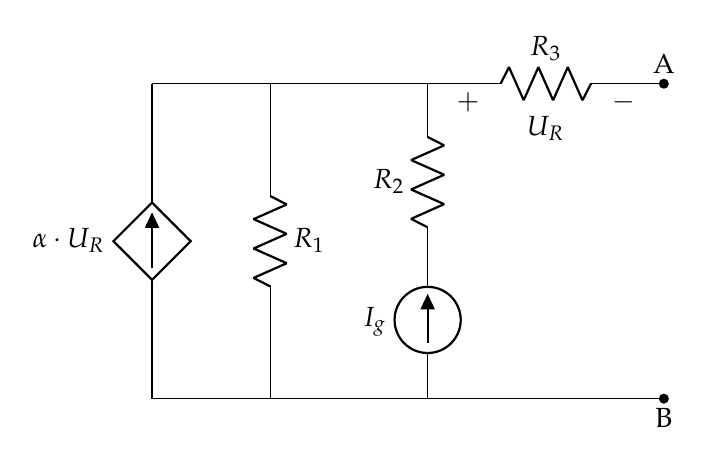
\begin{tikzpicture}
  \coordinate (A) at (0,0);
  \coordinate (B) at ($(A) + (1.5, 0)$) ;
  \coordinate (C) at ($(B) + (2, 0)$) ;
  \coordinate (D) at ($(C) + (3, 0)$) ;
  \coordinate (E) at ($(A) + (0, 4)$) ;
  \coordinate (F) at ($(B) + (0, 4)$) ;
  \coordinate (G) at ($(C) + (0, 4)$) ;
  \coordinate (H) at ($(D) + (0, 4)$) ;
  \draw
  (A) to [cI, l=$\alpha \cdot U_R$] (E)
  (B) to [R, l_ = $R_1$] (F)
  (C) to [isource, l=$I_g$] ++(0,2)
  to [R, l = $R_2$] ++(0,1.5)
  to [short] (G)
  to [R, l = $R_3$, -*, v = $U_R$] (H) node[above] {A}
  (A) to [short, -*] (D) node[below] {B}
  (E) to [short] (G);
\end{tikzpicture}
\end{document}